% Eingangsdaten der Simulation

\section{Modellbildung}

Grundlage für die Lastflussberechnung durch \edisgo bilden verschiedene Modelleingangsdaten.
Hierzu gehören in erster Linie die mit \simbev erzeugten Lastprofile der Ladevorgänge der \gls{EPKW}, die Topologie der \gls{MS}- und \gls{NS}-Netze, sowie die Erzeugungsprofile erneuerbarer Energieanlagen in einem Netzgebiet.
Weiterhin gehen auch die Lastprofile von Wärmepumpen in die Lastflussberechnung mit ein.
Dieses Kapitel soll einen Überblick über das verwendete Modell und die Eingangsdaten geben.\medskip


\subsection{Erzeugung der Lastzeitreihen der Ladevorgänge von E-Pkw}

% TODO: ding0

In diesem Kapitel wird auf die theoretischen Grundlagen und die simulative Erzeugung der Lastzeitreihen von \glspl{EPKW} eingegangen.
Die Lastzeitreihen der \glspl{EPKW} und die Optimierung dieser hin zu einem möglichst netzfreundlichen Verhalten, bilden den flexiblen Anteil der Eingangsdaten für die Lastflussberechnung mit \edisgo.\medskip

Mit Hilfe des im Rahmen dieser Masterarbeit mitentwickelten Software Tools \simbev können die Fahrtprofile für eine beliebige Anzahl an Fahrzeugen der verschiedenen Klassen für verschiedene Raumtypen erstellt werden (s. \autoref{chap:simbev_theo}.
Die Fahrtprofile enthalten die gefahrenen Strecken und die Standzeiten am Zielort.
Aus diesen können anschließend anhand des Verbrauchs und der gegebenen Ladeinfrastruktur die Ladebedarfe am Zielort abgeleitet werden.
Abhängig von der Ladestrategie wird die spezifische Last innerhalb der Standzeit verteilt.
Die Zeitreihen der Ladelast der einzelnen Fahrzeuge werden innerhalb eines Landkreises berechnet und schlussendlich zu einer Gesamtlast je \UC zusammengeführt.
Mit Hilfe des proprietär \localiserToolsKomma , werden die Zeitreihen der Gesamtlasten auf konkrete georeferenzierte Ladepunkte innerhalb des Landkreises verteilt.
Um abschließend eine Lasflussrechnung eines Netzgebietes mit \edisgo durchführen zu können, muss die Schnittmenge eines Netzgebietes mit den Landkreisen bestimmt werden.
Ladepunkte die innerhalb dieser Schnittmenge liegen, werden dem jeweiligen Netzgebiet zugeordnet und somit die entsprechende Last der Ladevorgänge.
Da die Simulation aller Netzgebiete zu inakzeptabel hohen Rechenzeiten führt, werden die \dingo Netzgebiete vorerst geclustert und Referenznetzgebiete identifiziert.


\subsubsection{Clustering der ding0 Netzgebiete}

% TODO: Auswertungen von Birgit übernehmen
% TODO: Karte mit den Netzgebieten
% TODO: welche charakteristischen Attribute wurden verwendet? @Birgit
% TODO: Schnittmenge Gemeinden <-> Netzgebiet erklären -> Karte!

Die Untersuchung der mit Hilfe des Software Tools \dingo synthetisierten \gls{MS}-Netzgebiete, führt aufgrund ihrer großen Anzahl zu inakzeptabel hohen Rechenzeiten während der Optimierung und Simulation.
Im Rahmen dieser Masterarbeit wurden sechs Referenznetzgebiete ausgewählt, welche einen Großteil der \num{3591} \gls{MS}-Netze repräsentieren.\medskip

Das Clustering erfolgt durch den während des \openego Projektes entwickelten k-means-Clusteralgorithmus (s. \autoref{chap:dingo_theo}).
Hierfür wurden die kumulierte Wind- und kumulierte Photovoltaikkapazität, sowie die kumulierte Last im Netzgebiet als charakteristische Attribute der \gls{MS}-Netze festgelegt.
Zusätzlich wurde überschlägig der zu erwartende Energiebedarf aufgrund der Eektromobilität im Elektrifizierungs-Szenario als Attribut festgelegt.

% TODO: Formel oder genauer erklären

Mit Hilfe 


\subsubsection{Erstellung der Fahrtprofile mit simBEV}

Mit Hilfe des Software Tools \simbev (s. \autoref{chap:simbev_theo}) können für die zuvor geclusterten Referenznetzgebiet die entsprechenden Fahrtprofile der im Netzgebiet befindlichen Fahrzeuge erzeugt werden.
Um die Anzahl an Fahrzeugen je Netzgebiet zu bestimmen, muss der Gesamtbestand an Fahrzeugen je Szenario (s. \autoref{tab:SzenarienRampUp} und \autoref{tab:CarSplit}) regionalisiert werden.
Die Regionalisierung der Fahrzeuge findet vorerst auf Ebene der Landkreise statt.
Als Grundlage hierfür dient der aktuelle Fahrzeugbestand nach Zulassungsbezirken \cite[][Stand: \DTMdate{2020-01-01}]{KBAPLZ2020}.
Es wird davon ausgegangen, dass es zu keiner Verschiebung des Anteils am Bestand zwischen den Zulassungsbezirken kommt.
Dies bedeutet, dass die Gesamtanzahl der Fahrzeuge je Fahrzeugklasse je Szenario entsprechend des heutigen Bestandes anteilig verteilt wird.
Die Aufteilung der Fahrzeuge in Klassen erfolgt anhand der Einteilung des Fahrzeugsbestands in Hubraum-Klassen, welche ebenfalls dem Fahrzeugbestand nach Zulassungsbezirken entnommen werden können.\medskip

Die Einteilung der \Regiostar Raumtypen erfolgt auf Gemeindeebene, weshalb eine weitere Regionalisierung der Fahrzeuge innerhalb eines Landkreises auf die jeweiligen Gemeinden nötig ist.
Da auf Gemeindeebene keine Daten zum Fahrzeugbestand vorliegen, erfolgt die Regionalisierung anhand der Einwohnerzahl der Gemeinden.
Die Grundlage hierfür bildet der Datensatz \glqq Gemeindegrenzen 2017 mit Einwohnerzahl\grqq{} \cite[][Stand: \DTMdate{2017-12-31}]{EDG2020}.
Die Verteilung der Anzahl der Fahrzeuge erfolgt streng proportional zur Einwohnerzahl in der jeweiligen Gemeinde.\medskip

Um abschließend die Fahrtprofile erzeugen zu können, muss jeder Gemeinde ein \Regiostar Raumtyp zugeordnet werden.
Die entsprechende Zuordnung für das Jahr \num{2018} kann dem Datensatz \glqq Referenzdateien zur regionalstatistischen Raumtypologie\grqq{} \cite[][Stand: \DTMdate{2018-01-01}]{BMVIa2020} entnommen werden.


\subsubsection{Charakteristik der Fahrtprofile}
% TODO: Fahrtstrecke berechnen mean +- Standardabweichung

Die Charakteristik der Fahrtprofile spielt eine entscheidende Rolle für die Wirksamkeit der unterschiedlichen Ladestrategien und die Auswirkungen auf die Netze.
Hierbei steht vor allem der Anteil flexibilisierbarer und nicht-flexibilisierer Ladevorgänge, sowie die Gleichzeitigkeit von Ladevorgängen im Vordergrund.\medskip

Der Anteil flexibilisierbarer Ladevorgänge entspricht dem Anteil am Gesamtenergiebedarf, der an privaten Ladepunkten zu Hause oder am Arbeitsplatz nachgeladen wird.
Hierzu zählen alle Ladevorgänge die am Eigenheim, einer Wohnaalage oder auf einem Firmenparkplatz stattfinden.
Demgegenüber stehen nicht-flexibilisierer Ladevorgänge im öffentlichen Raum und an Schnellladestationen.
Je nach Raumtypen unterscheidet sich das Verhältnis leicht.
Im Mittel liegt der Anteil nicht-flexibilisierer Ladevorgänge über alle Szenarien innerhalb der einzelnen Gemeinden bei \SI{30}{\percent}.
Hiervon ausgenommen ist die \SzeFirmenparkplatzdot, bei der es aufgrund des geringeren Bestands an Ladeinfrastruktur am Arbeitsplatz zu mehr Ladevorgängen im öffentlichen Raum kommt.
Der Anteil nicht-flexibilisierer Ladevorgänge liegt bei dieser Szenarette bei \SI{40}{\percent}.
In \autoref{tab:ChargingShare} findet sich die entsprechende Aufteilung.

{
\renewcommand{\arraystretch}{1.2}% grßerer Zeilenabstand
\sisetup{range-phrase=~{--}~}% Gedankenstrich statt "bis" bei SIrange
\begin{table}[H]
	\begin{center}
		\caption{Aufteilung in flexibiliserbare und nicht-flexibiliserbare Ladevorgänge}
		\begin{tabu} to \textwidth {X[1] X[1, r] X[1, r]}
			\hline
								  & \SzeFirmenparkplatzdot                              & Sonstige Szenarien                                  \\ \hline
			Flexibiliserbar       & \SI[separate-uncertainty = true]{70.0(24)}{\percent} & \SI[separate-uncertainty = true]{75.2(14)}{\percent} \\
			Nicht-flexibiliserbar & \SI[separate-uncertainty = true]{30.0(24)}{\percent} & \SI[separate-uncertainty = true]{24.8(14)}{\percent} \\ \hline
			\multicolumn{3}{l}{Angabe als Anteil   vom Gesamtenergiebedarf der Fahrzeuge}
		\end{tabu}
		\label{tab:ChargingShare}
	\end{center}
	\vspace{-3mm}%Put here to reduce too much white space after your table
\end{table}
}

In \autoref{fig:example_load_profile} findet sich stellvertretend das \gls{EV}-Lastprofil für ungesteuertes Laden einer mittelstädtischen Gemeinde mit \num{6443} \glspl{EV} über eine Woche im Elektrifizierungs-Szenario (links).
Zusätzlich wurde die \SzeFirmenparkplatz (rechts) dargestellt.

\begin{figure}[H]
    \centering
    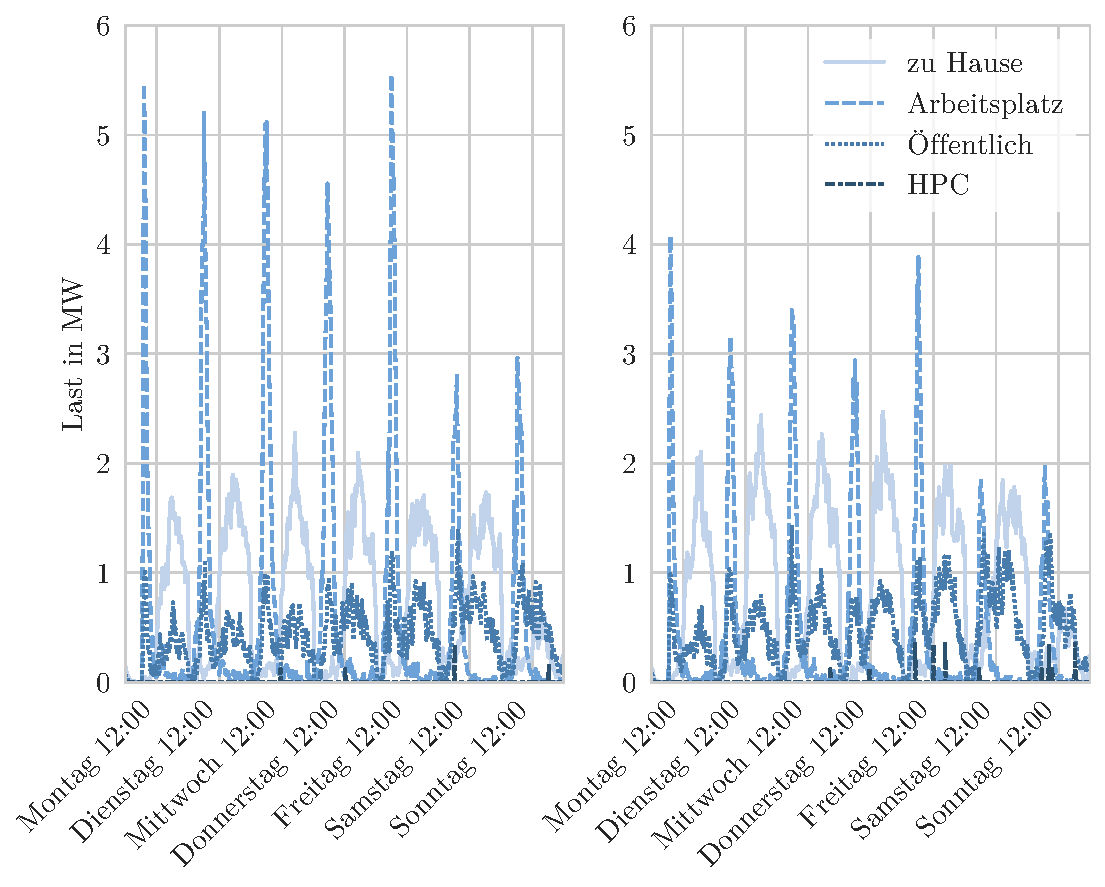
\includegraphics[width=\textwidth]{Bilder/example_load_profile}
    \caption{EV-Lastprofil für ungesteuertes Laden einer mittelstädtischen Gemeinde mit \num{6443} \glspl{EV} über eine Woche im Elektrifizierungs-Szenario (links) und der \SzeFirmenparkplatz (rechts)}\label{fig:example_load_profile}
\end{figure}

Die Lastgänge \zH und \Firmeparkplatz entsprechen den flexibilisierbaren Ladevorgängen im privaten Bereich. Unter dem Lastgang \oeffen sind hingegen alle öffentlichen Ladevorgänge mit Außnahme der Schnellladevorgänge (\gls{HPC}) zusammengefasst. Deutlich zu erkennen ist die hohe Gleichzeitigkeit am Vormittag sowohl am \Firmeparkplatz als auch im öffentlichen Raum, welche durch das Fahren zur Arbeit ausgelöst wird.
Auch die Rückkehr zum Wohnort ist ab dem frühen Nachmittag in den Lastgängen \zH und im öffentlichen Raum deutlich zu erkennen. Die entsprechenden Dauerlastkurven für die Gemeinde über die gleiche Woche (s. \autoref{fig:example_load_curve}) zeigen dies nochmals deutlich.
Schnellladevorgänge werden hingegen vermehrt am Wochenende ausgelöst, da verstärkt längere Fahrten angetreten werden.
Am Wochenende kommt es zusätzlich zu deutlich geringeren Anteilen von Ladevorgängen \zH und am \Firmeparkplatzdot, wodurch das Flexibilisierungspotential am Wochenende geringer ausfällt.
Gegenüber dem Elektrifizierungs-Szenario sinkt die Höchstlast in der \SzeFirmenparkplatzdot, jedoch sinkt auch das Flexibilisierungspotential bei gleichbleibendem Energiebedarf durch die Verschiebung der Ladevorgänge in den öffentlichen Raum.

\begin{figure}[H]
    \centering
    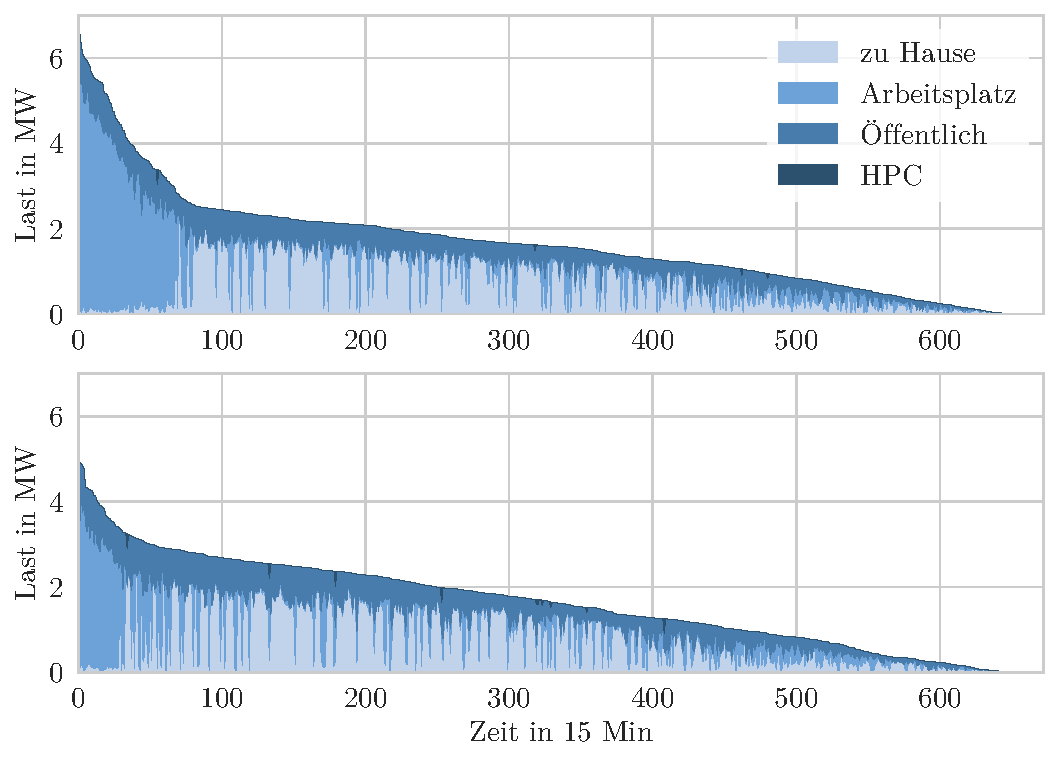
\includegraphics[width=\textwidth]{Bilder/example_load_duration_curve}
    \caption{EV-Dauerlastkurve für ungesteuertes Laden einer mittelstädtischen Gemeinde mit \num{6443} \glspl{EV} über eine Woche im Elektrifizierungs-Szenario (oben) und der \SzeFirmenparkplatz (unten
    )}\label{fig:example_load_curve}
\end{figure}


\subsubsection{Kritik}

Die erstellten Fahrtprofile spiegeln ein aus heutiger Sicht plausibel erscheinendes Bild wider.
Dennoch existieren einzelne Kritikpunkte, die innerhalb des \simbev Projektes gelöst werden sollten.
So war es zum Zeitpunkt der Erstellung der Fahrtprofile noch nicht möglich, einen längeren Zeitraum als eine Woche am Stück zu simulieren.
Da sich jedoch die Netzuntersuchungen im Rahmen dieser Masterarbeit auf einen Zeitraum von einem Jahr beziehen, wird die simulierte Woche stellvertretend für das gesamte Jahr verwendet.
Hierfür wurde jedes Fahrtprofil solange mit sich selbst verlängert und logisch verknüpft, bis die gewünschte Länge erreicht wurde.
Dieses bringt jedoch einige Nachteile mit sich.
Durch den kurzen simulierten Zeitraum fällt der \gls{SOC} einiger Fahrzeuge im Laufe der Woche nur geringfügig.
Es ist zu vermuten, dass dies dazu führt, dass Ladevorgänge an Schnellladeinfrastruktur un­ter­re­prä­sen­tiert dargestellt werden.
Auch nimmt der Ladebedarf im öffentlichen Raum im Laufe der Woche zu.
Dies lässt sich durch die Abhängigkeit der Ladewahrscheinlichkeit vom \gls{SOC} erklären, da der \gls{SOC} im Mittel im Verlaufe des Woche sinkt.


\subsection{Localiser Tool}


\subsection{eDisGo}

\subsubsection{Implementierung der Ladestrategien}

\subsubsection{Lastflussberechnung}